\chapter{Intervals}

\classquote{夫和实生物，同则不继。以他平他谓之和，故能丰长而物归之；若以同裨同，尽乃弃矣。\\
Harmony brings things into being; sameness does not continue. To set one thing beside another and balance them is called harmony; thus things grow and come home. If one piles sameness on sameness, when it is exhausted, it is thrown away.}{Discourses of the States · Discourses of Zheng}{Two different pitches must balance each other before there is “harmony”; piling the same pitch on itself soon runs out. An interval is exactly that distance between “others”, and different distances carry different tension and release.}

\label{sec:intervals}

\section*{What you can do after this chapter}
\begin{itemize}
  \item Given two note names, say how many semitones separate them and what interval they form (C4--E4 is a major third).
  \item Separate the ``number'' of an interval from its ``quality,'' and stop confusing ``a third'' with ``three semitones.''
  \item Judge common intervals as consonant or dissonant, and know that the same interval can change function with harmonic context.
  \item Measure two notes' row distance in Yeban's piano roll and use transposition plus playback for interval-ear training.
\end{itemize}

\section{Semitone: the distance unit of intervals}

An interval is the pitch distance between two notes. Its most concrete unit is the semitone: on a piano, adjacent keys (including black keys) are a semitone apart; in the piano roll, adjacent rows are a semitone apart. A whole tone is two semitones.

Semitone count alone is not enough. C4--E4 is four semitones, and C4--F\flatsym4 is also four semitones, yet the first is a major third and the second a diminished fourth; in equal temperament they sound the same, but their spelling and harmonic meaning differ. A complete interval name therefore has two parts:

\begin{itemize}
  \item \textbf{Quantity}: count from the first note to the second, including both ends. C--D is a second, C--E a third, C--G a fifth, C--C (an octave up) an octave.
  \item \textbf{Quality}: major, minor, perfect, augmented, or diminished; it describes the semitone difference within the same quantity.
\end{itemize}

\begin{center}
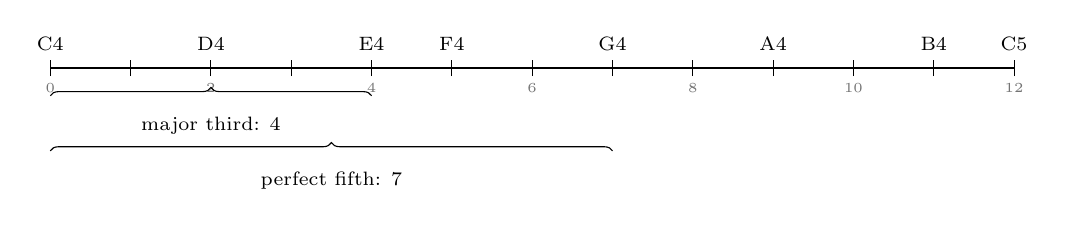
\begin{tikzpicture}[x=1.02cm,y=1cm,font=\scriptsize]
  \draw[thick] (0,0) -- (12,0);
  \foreach \i in {0,...,12} {\draw (\i,-0.1) -- (\i,0.1);}
  \foreach \i/\n in {0/C4,2/D4,4/E4,5/F4,7/G4,9/A4,11/B4,12/C5} {
    \node[above=3pt] at (\i,0) {\n};
  }
  \foreach \i in {0,2,...,12} {\node[below=2pt,font=\tiny,text=black!55] at (\i,0) {\i};}
  \draw[decorate,decoration={brace,amplitude=3pt}] (0,-0.35) -- (4,-0.35)
    node[midway,below=4pt] {major third: 4};
  \draw[decorate,decoration={brace,amplitude=3pt}] (0,-1.05) -- (7,-1.05)
    node[midway,below=4pt] {perfect fifth: 7};
\end{tikzpicture}

\small Figure 3-1. A semitone ruler from C4 to C5. Numbers below every second tick are semitone counts; quantity counts both ends, quality compares semitones within the same quantity.
\end{center}

\section{Counting the quantity and fixing the quality}

Always include the starting note when counting the quantity: C to E is C(1), D(2), E(3), a third. Counting only the notes ``in between'' gives one too few. The octave works the same way: C4 to C5 spans eight letter names including both ends, so it is an octave, not a seventh.

Quality uses the natural major scale as its reference. In C major:

\begin{itemize}
  \item C--D, C--E, C--A, C--B are major second, major third, major sixth, major seventh.
  \item Lower a major interval by one semitone and it becomes minor: C--E\flatsym{} is a minor third, C--A\flatsym{} a minor sixth.
  \item Unison, fourth, fifth, and octave use ``perfect'': C--C is a perfect unison, C--F a perfect fourth, C--G a perfect fifth, C--C (octave) a perfect octave.
  \item Widen a perfect interval by a semitone to get augmented, narrow it by a semitone to get diminished; the same words apply when widening/narrowing major/minor intervals.
\end{itemize}

\begin{center}
\small
\begin{tabular}{llcl}
\toprule
Interval & Semitones & Example from C4 & Quality \\
\midrule
minor second & 1 & C4--D\flatsym4 & minor \\
major second & 2 & C4--D4 & major \\
minor third & 3 & C4--E\flatsym4 & minor \\
major third & 4 & C4--E4 & major \\
perfect fourth & 5 & C4--F4 & perfect \\
augmented fourth / diminished fifth & 6 & C4--F\sharpsym4 / C4--G\flatsym4 & aug. / dim. (tritone) \\
perfect fifth & 7 & C4--G4 & perfect \\
minor sixth & 8 & C4--A\flatsym4 & minor \\
major sixth & 9 & C4--A4 & major \\
minor seventh & 10 & C4--B\flatsym4 & minor \\
major seventh & 11 & C4--B4 & major \\
perfect octave & 12 & C4--C5 & perfect \\
\bottomrule
\end{tabular}

Table 3-1. The twelve basic intervals within an octave. The six-semitone tritone has two enharmonic spellings: augmented fourth and diminished fifth.
\end{center}

Intervals larger than an octave are compound: a ninth is an octave plus a second, a tenth an octave plus a third. You can say ``major ninth'' or ``an octave plus a major second''; both describe the same pitch relationship.

\section{Consonance and dissonance}

Consonance and dissonance are listening categories, not moral judgments. A common convention:

\begin{itemize}
  \item \textbf{Perfect consonance}: perfect unison, octave, fifth; the perfect fourth is traditionally classed as perfect consonance, but in modern listening/orchestration it is sometimes heard as a ``tense fourth,'' depending on context.
  \item \textbf{Imperfect consonance}: major/minor thirds and sixths. They carry more color than perfect consonances yet still blend easily.
  \item \textbf{Dissonance}: seconds, sevenths, and the tritone. They create tension that usually wants resolution, or is deliberately sustained.
\end{itemize}

``Dissonant'' does not mean ``bad.'' Cymbal crashes, distorted guitars, and film-score tritones all use dissonance as color. The test is whether the tension is resolved later and whether it serves the section's emotion, not a lookup table alone.

\section{Inversion and enharmonic spelling}

Moving the lower note of an interval above the upper note (or vice versa) is an inversion. The quantity becomes ``9 minus the original quantity,'' and the quality usually flips:

\begin{itemize}
  \item major second $\leftrightarrow$ minor seventh; minor third $\leftrightarrow$ major sixth; major third $\leftrightarrow$ minor sixth; major seventh $\leftrightarrow$ minor second.
  \item perfect fourth $\leftrightarrow$ perfect fifth; perfect octave $\leftrightarrow$ perfect unison; augmented fourth $\leftrightarrow$ diminished fifth.
\end{itemize}

\begin{figure}[htbp]
\centering
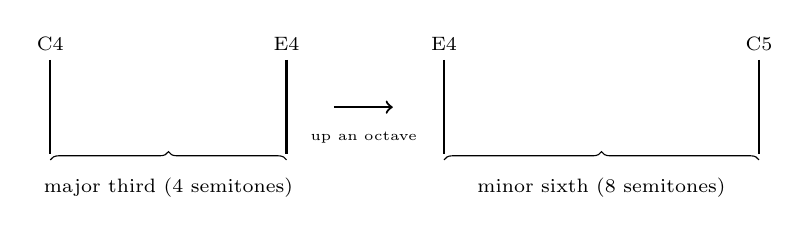
\begin{tikzpicture}[x=1cm,y=1cm,font=\scriptsize]
  \draw[thick] (0,2.2) -- (0,1.0);
  \draw[thick] (3,2.2) -- (3,1.0);
  \node[above] at (0,2.2) {C4};
  \node[above] at (3,2.2) {E4};
  \draw[decorate,decoration={brace,amplitude=3pt},yshift=-2pt] (0,1.0) -- (3,1.0)
    node[midway,below=3pt] {major third (4 semitones)};

  \draw[->,thick] (3.6,1.6) -- (4.35,1.6);
  \node[below=1pt,font=\tiny] at (3.98,1.45) {up an octave};
  \draw[thick] (5,2.2) -- (5,1.0);
  \draw[thick] (9,2.2) -- (9,1.0);
  \node[above] at (5,2.2) {E4};
  \node[above] at (9,2.2) {C5};
  \draw[decorate,decoration={brace,amplitude=3pt},yshift=-2pt] (5,1.0) -- (9,1.0)
    node[midway,below=3pt] {minor sixth (8 semitones)};
\end{tikzpicture}

\small Figure 3-2. C4--E4 (major third) inverts to E4--C5 (minor sixth); quantities 3 + 6 = 9, semitones 4 + 8 = 12.
\end{figure}

Enharmonic spelling is a different matter: the same key/pitch written with different note names. C\sharpsym{} and D\flatsym{} are enharmonic; an augmented fourth C--F\sharpsym{} and a diminished fifth C--G\flatsym{} are enharmonic intervals. In equal temperament their frequencies match, but in notation, chord function, and melody writing they are not interchangeable: whether you write F\sharpsym{} or G\flatsym{} depends on the note it must resolve to.

\section{Hearing and singing intervals}

Do not start interval ear training by memorizing a table; build references first:

\begin{enumerate}
  \item Calibrate with a familiar octave: C4 to C5 is twelve semitones, double the frequency.
  \item Then hear a perfect fifth (seven semitones) and a perfect fourth (five); they are the two most stable intervals outside the octave.
  \item A major third (four semitones) and a minor third (three) differ by one semitone, yet the color difference is ``bright'' versus ``soft''; play C--E and C--E\flatsym{} from the same root.
  \item Finally practice dissonance: major second, minor seventh, tritone. Do not rush to call it ``wrong''; first hear whether it wants resolution.
\end{enumerate}

When singing intervals, go from root to target with either movable or fixed solfège, but always start from the same root; reverse it for descending. Melodic intervals (notes one after another) are easier than harmonic intervals (notes together), so practice melodic first, then harmonic.

\section{How to do it in Yeban}

\begin{enumerate}
  \item Open the piano roll (\texttt{P}/\texttt{F7}) and write a note on the C4 row, then another on E4. Adjacent rows are semitones, so the row distance is the semitone count: C4 to E4 is four rows.
  \item For a melodic interval, offset the two notes in time; for a harmonic interval, put them on the same beat. Press \texttt{Space} and first judge ``consonant/dissonant,'' then check the row distance against the interval name.
  \item Select the upper note and use \texttt{↓} or \texttt{Shift+↓} to transpose. Each semitone can change quality from major to minor, or from perfect to augmented/diminished. Use this to turn C4--E4 into C4--E\flatsym4 (minor third) and C4--F4 (perfect fourth), and listen.
  \item Invert: select the lower C4 and press \texttt{Shift+↑} to raise it an octave to C5; C4--E4 becomes E4--C5 (minor sixth), and the row distance goes from 4 to 8, confirming ``quantities add to 9.''
  \item For finer ear training, use A4 = 440 Hz as a reference and compare the target to A4; do not judge from memory without calibrating tempo and monitoring.
\end{enumerate}

\screenshot{piano-roll-interval-two-notes}{Two notes and their interval spacing in the piano roll}{Two notes and their interval spacing in the piano roll}

\textbf{Scope note:} Yeban does not currently provide automatic interval recognition or ear-training scoring. This chapter's ear training relies on the ear plus row-distance checking, not on an analysis button that does not exist. If one is added later, this section will link to it.

\section{Emotional intervals in real songs}

\begin{itemize}
  \item \textbf{Judy Garland, ``Over the Rainbow''}: Opens with an ascending \textbf{perfect octave} on ``Some-where'', instantly opening vertical space and longing.
  \item \textbf{John Williams, ``Jaws'' theme}: Alternates a single low-register \textbf{minor second} (one semitone) and accelerates it, showing that the smallest interval can build the sharpest tension.
  \item \textbf{John Williams, ``Star Wars'' main theme}: Launches with an ascending \textbf{perfect fifth} (C$\rightarrow$G) that projects heroic clarity in two notes.
\end{itemize}

\section{Exercises}


\begin{exercise}
\begin{enumerate}
  \item What quantity and how many semitones is C4--G4? What quality?\\
  \emph{Answer:} A fifth, seven semitones, perfect fifth.
  \item How many semitones separate C4--A4 and C4--A\flatsym4? What are they?\\
  \emph{Answer:} One semitone; C4--A4 is a major sixth (9 semitones), C4--A\flatsym4 a minor sixth (8 semitones).
  \item What does a major third invert to, and how do the semitones change?\\
  \emph{Answer:} A minor sixth; four semitones become eight.
  \item Why do an augmented fourth and a diminished fifth sound the same but cannot be freely swapped in notation?\\
  \emph{Answer:} In equal temperament they are enharmonic (both six semitones), but their notation, function, and resolution direction differ; swapping changes harmonic meaning.
  \item In Yeban, write C4--E4 and listen to the harmonic interval; then lower E4 to E\flatsym4 and hear the color difference between major and minor thirds.\\
  \emph{Hint:} Align to the C4 and E4 rows and confirm a four-row distance; after lowering, the distance becomes three.
\end{enumerate}
\end{exercise}

\section{Help topic map}

\begin{center}
\footnotesize
\setlength{\tabcolsep}{3pt}
\begin{longtable}{p{0.33\linewidth}p{0.44\linewidth}p{0.17\linewidth}}
\toprule
Section & In-app help anchor & Note \\
\midrule
\endhead
Semitone and interval distance & \texttt{music-theory-semitone-distance} & Figure 3-1 \\
Quantity and quality & \texttt{music-theory-interval-quantity-quality} & Table 3-1 \\
Consonance and dissonance & \texttt{music-theory-consonance-dissonance} & concept \\
Inversion and enharmonic spelling & \texttt{music-theory-inversion-enharmonic} & Figure 3-2 \\
Hearing and singing intervals & \texttt{music-theory-interval-ear-training} & practice method \\
How to do it in Yeban & \texttt{music-theory-piano-roll-intervals} & procedure \\
Exercises & \texttt{music-theory-ch3-practice} & answers above \\
\bottomrule
\end{longtable}
\end{center}

\section*{Further reading}
\begin{itemize}
  \item \textbf{Open Music Theory, “Intervals.”} \url{https://openmusictheory.github.io/intervals.html} — covers size, quality, inversion, and consonance, the calculation rules behind this chapter.
  \item \textbf{YouTube, “Listening to intervals.”} \url{https://www.youtube.com/watch?v=VHQO_E17Yhk} — trains the ear with melody anchors so intervals become audible distances.
\end{itemize}

